\section{Optimal Labor Supply}


We consider a static equilibrium with heterogeneous ability. There is a continuum of households indexed by ability $e \in [1,\bar{e}]$, distributed according to a truncated Pareto distribution $e \sim \widehat{F}(e)$. Each household chooses hours $h \ge 0$ to maximize CRRA utility separable in labor and consumption, subject to a budget constraint. Production is Cobb--Douglas in aggregate labor, with decreasing returns to scale, and the government levies a linear tax on labor income and rebates revenue lump-sum.

The goal is to compute the equilibrium allocation: a wage $W$, a lump-sum transfer $T$, and a schedule of hours $h(e)$ and consumption $c(e)$ such that (i) households optimize, (ii) firms maximize profits, and (iii) the goods market clears.

\subsection{Setup}

Ability is distributed with truncated Pareto cdf $\widehat{F}(e) = (1 - e^{-\alpha}) / (1 - \bar{e}^{-\alpha})$ on $[1,\bar{e}]$. We discretize this distribution using Gauss--Legendre quadrature: nodes $\{e_i\}_{i=1}^n$ and weights $\{\omega_i\}_{i=1}^n$ with $\sum_i \omega_i = 1$, so that expectations are approximated by $\E[g(e)] \approx \sum_i \omega_i g(e_i)$. Aggregate labor supply is
\begin{equation}
  L = \sum_{i=1}^n \omega_i e_i h_i.
\end{equation}
Output is $Y = L^\eta$ with $\eta \in (0,1)$. Under perfect competition, the wage is
\begin{equation}
  W = \eta L^{\eta - 1}.
\end{equation}
Tax revenue is rebated lump-sum; with tax rate $\tau$ on labor income, the transfer is
\begin{equation}
  T = L^\eta - (1-\tau) W L.
\end{equation}
Household $i$ has consumption
\begin{equation}
  c_i = T + (1-\tau) W e_i h_i.
\end{equation}
With CRRA utility in consumption and disutility of labor, the first-order condition for interior $h_i > 0$ is
\begin{equation}
  h_i^\gamma = (1-\tau) W e_i c_i^{-\sigma}.
\end{equation}

\subsubsection{System of equations}

Collect the vector of hours $\mathbf{h} = (h_1,\ldots,h_n)^\top$. Define aggregate objects as functions of $\mathbf{h}$:
\begin{align}
\begin{split}
  L(\mathbf{h}) &= \sum_{i=1}^n \omega_i e_i h_i, \\
  W(\mathbf{h}) &= \eta L(\mathbf{h})^{\eta-1}, \\
  T(\mathbf{h}) &= L(\mathbf{h})^\eta - (1-\tau) W(\mathbf{h}) L(\mathbf{h}).
\end{split}
\end{align}
Consumption of household $i$ is $c_i(\mathbf{h}) = T(\mathbf{h}) + (1-\tau) W(\mathbf{h}) e_i h_i$. The residual for the FOC of household $i$ is
\begin{equation}
  F_i(\mathbf{h}) = h_i^\gamma - (1-\tau) W(\mathbf{h}) e_i c_i(\mathbf{h})^{-\sigma}.
\end{equation}
Equilibrium is a root of the $n$-dimensional system
\begin{equation}
  \mathbf{F}(\mathbf{h}) = \mathbf{0}.
\end{equation}
Goods market clearing is implied: $\sum_i \omega_i c_i = Y = L^\eta$ at a solution.

\subsection{Solution methods}

We implement two approaches: (1) solve $\mathbf{F}(\mathbf{h})=\mathbf{0}$ in one shot with a robust Broyden method; (2) solve by fixed point on the wage $W$, with an inner Broyden step for the vector of hours given $W$.

\subsubsection{Approach 1: Full system (Broyden on $\mathbf{F}$)}

We solve the coupled system $\mathbf{F}(\mathbf{h})=\mathbf{0}$ directly. Because the Jacobian of $\mathbf{F}$ is dense and the system can be ill-scaled, we use the CompEcon-style Broyden method (inverse Jacobian approximation, backstepping line search, restarts), i.e.\ \texttt{broyden(..., method='compecon')}.

\begin{algorithm}[H]
\caption{Full-system Broyden for labor supply equilibrium}
\label{alg:broyden-full}
\begin{algorithmic}[1]
\State \textbf{Input:} Residual $\mathbf{F}$, initial guess $\mathbf{h}^{(0)}$, tolerance $\varepsilon$, max iterations $K$
\State \textbf{Output:} Equilibrium hours $\mathbf{h}^*$
\State $k \gets 0$
\While{$k < K$ and $\|\mathbf{F}(\mathbf{h}^{(k)})\|_\infty > \varepsilon$}
  \State Update $\mathbf{h}^{(k+1)}$ via Broyden (inverse Jacobian + line search)
  \State $k \gets k + 1$
\EndWhile
\State \textbf{return} $\mathbf{h}^{(k)}$
\end{algorithmic}
\end{algorithm}

\subsubsection{Approach 2: Fixed point on wages (inner componentwise Broyden)}

Given a guess for the wage $W$, the transfer is $T = L^\eta - (1-\tau) W L$ with $L = \sum_i \omega_i e_i h_i$. For fixed $W$ and $T$, each household's FOC is a scalar equation in $h_i$ with bounds $0 \le h_i \le \bar{h}$. We solve this vectorized system with safeguarded componentwise Broyden, i.e.\ \texttt{broyden(..., method='componentwise', a=0, b=}$\bar{h}$\texttt{)}. Then we aggregate $L$, update $W \leftarrow \eta L^{\eta-1}$ (optionally damped), and repeat until $W$ converges.

\begin{algorithm}[H]
\caption{Wage fixed-point with inner componentwise Broyden}
\label{alg:wage-fp}
\begin{algorithmic}[1]
\State \textbf{Input:} Parameters $(\tau,\eta,\sigma,\gamma)$, quadrature $(e_i,\omega_i)$, bounds $(\underline{h},\bar{h})$, tolerance $\varepsilon$, max outer iterations $K_{\mathrm{out}}$, max inner iterations $K_{\mathrm{in}}$
\State \textbf{Output:} Equilibrium wage $W^*$ and hours $\mathbf{h}^*$
\State $W \gets W^{(0)}$ (e.g.\ initial guess)
\State $\mathbf{h} \gets \mathbf{h}^{(0)}$ (e.g.\ $\mathbf{1}$)
\For{$k = 1$ to $K_{\mathrm{out}}$}
  \State $L \gets \sum_i \omega_i e_i h_i$; \; $T \gets L^\eta - (1-\tau) W L$
  \State Solve for $\mathbf{h}$: FOC residuals in $h_i$ given $(W,T)$ equal zero, with $a_i = \underline{h}$, $b_i = \bar{h}$, using componentwise Broyden (max $K_{\mathrm{in}}$ iterations)
  \State $L_{\mathrm{new}} \gets \sum_i \omega_i e_i h_i$; \; $W_{\mathrm{new}} \gets \eta L_{\mathrm{new}}^{\eta-1}$
  \If{$|W_{\mathrm{new}} - W| < \varepsilon$}
    \State \textbf{return} $W_{\mathrm{new}}$, $\mathbf{h}$
  \EndIf
  \State $W \gets W + \lambda (W_{\mathrm{new}} - W)$ (damping $\lambda \in (0,1]$ optional)
\EndFor
\State \textbf{return} $W$, $\mathbf{h}$
\end{algorithmic}
\end{algorithm}

\begin{figure}[H]
\centering
\subfloat[Broyden iteration trace]{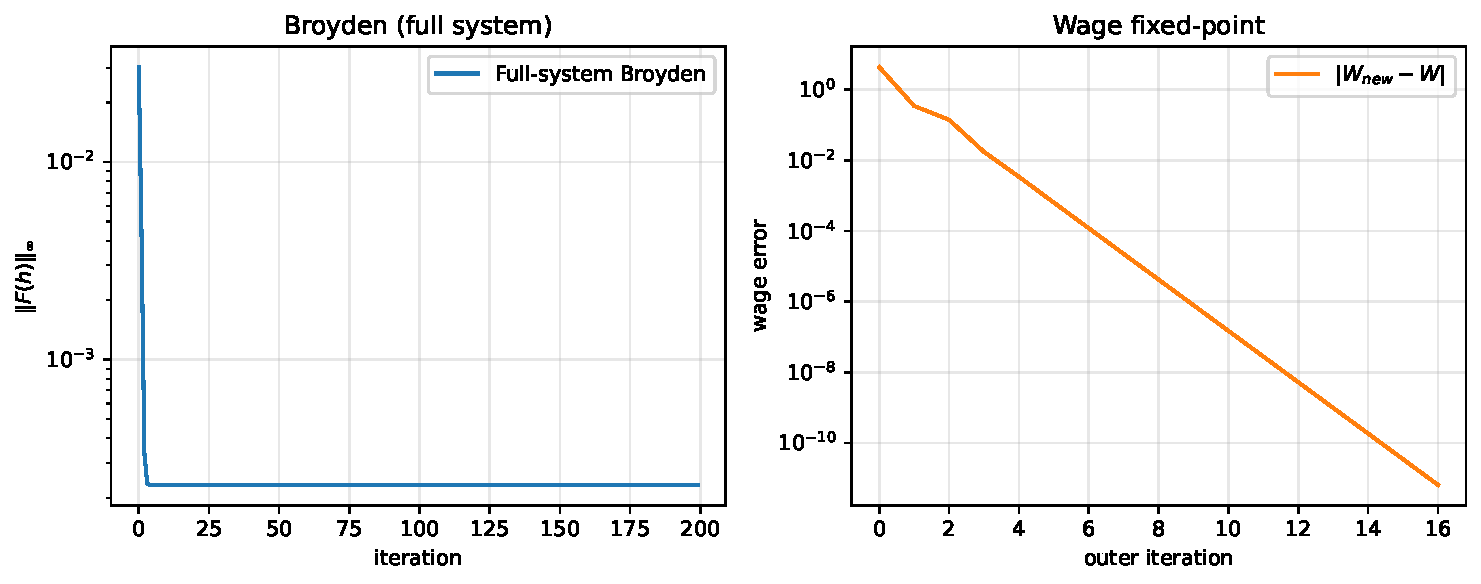
\includegraphics[width=0.48\textwidth]{figures/problem2_broyden_trace}}
\hfill
\subfloat[Equilibrium labor curve]{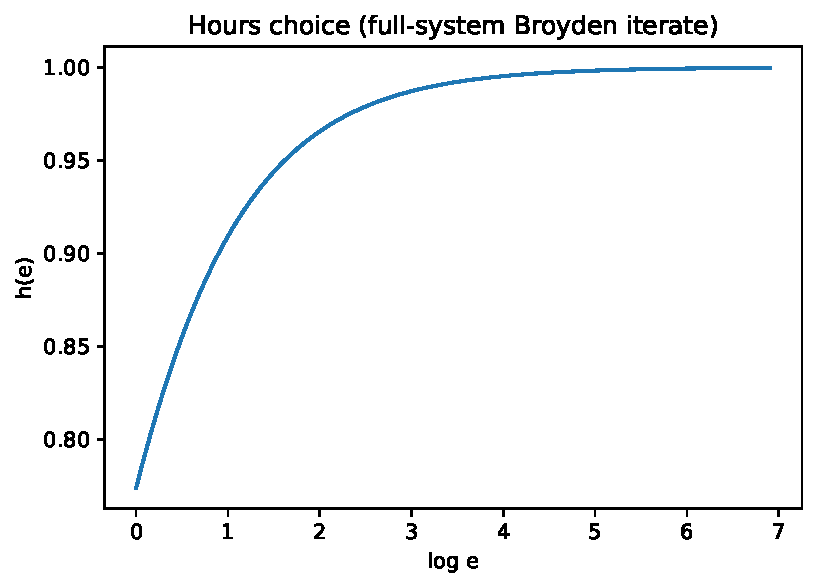
\includegraphics[width=0.48\textwidth]{figures/problem2_labor_curve}}
\caption{Broyden convergence (Approach 1: full-system CompEcon-style) and equilibrium hours $h(e)$ vs.\ $\log e$.}
\label{fig:problem2-results}
\end{figure}

\subsection{Implementation notes}

\begin{itemize}[leftmargin=*]
  \item \textbf{Quadrature (Sec.\ 2.1):} We use Gauss--Legendre nodes and weights on $[1,\bar{e}]$ and multiply weights by the truncated Pareto pdf so that $\sum_i \omega_i = 1$. We check that the first three moments match the analytical formulas.
  \item \textbf{Approach 1:} We call \texttt{broyden(..., method='compecon')} with guardrails in the residual (clip $h$ to $[10^{-12},\bar{h}]$, penalize $c \le 0$) to avoid numerical explosions.
  \item \textbf{Approach 2:} We call \texttt{broyden(..., method='componentwise', a=hmin, b=hmax)} for the inner FOC system given $(W,T)$. The outer loop updates $W$ until $|W_{\mathrm{new}} - W| < \varepsilon$.
  \item \textbf{Checks:} We verify goods market clearing $\sum_i \omega_i c_i = L^\eta$ and report the FOC residual norm and transfer $T$, labor $L$, output $Y$, and wage $W$.
\end{itemize}

% \subsection*{Pause / check}
% \begin{itemize}[leftmargin=*]
%   \item Check quadrature weights sum to 1 and moments match formulas.
%   \item Check goods market: $\sum_i \omega_i c_i = L^\eta$.
% \end{itemize}